% =========================================================
% Dirichlet Approximation – Pigeonhole Diagram
% =========================================================

\begin{figure}[h]
\centering
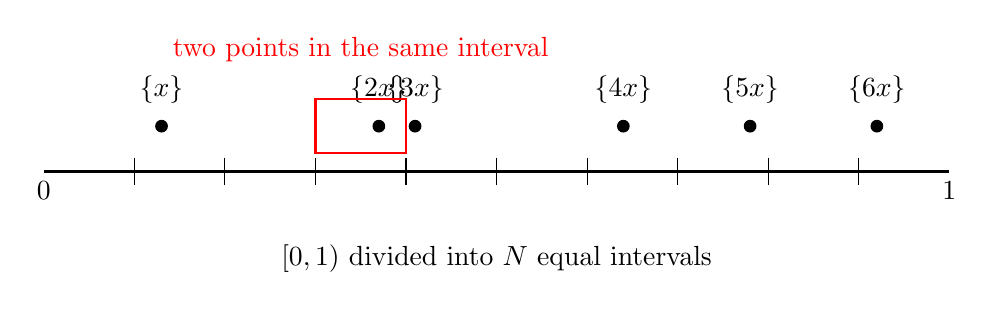
\begin{tikzpicture}[scale=1.15]

% Unit interval
\draw[thick] (0,0) -- (10,0);

% Endpoints
\node[below] at (0,0) {$0$};
\node[below] at (10,0) {$1$};

% Tick marks dividing into N intervals
\foreach \x in {1,2,3,4,5,6,7,8,9}
{
\draw (\x,0.15) -- (\x,-0.15);
}

\node[below] at (5,-0.7) {$[0,1)$ divided into $N$ equal intervals};

% Example points (fractional parts)
\fill (1.3,0.5) circle (2pt);
\fill (3.7,0.5) circle (2pt);
\fill (4.1,0.5) circle (2pt);
\fill (6.4,0.5) circle (2pt);
\fill (7.8,0.5) circle (2pt);
\fill (9.2,0.5) circle (2pt);

% Labels
\node at (1.3,0.9) {$\{x\}$};
\node at (3.7,0.9) {$\{2x\}$};
\node at (4.1,0.9) {$\{3x\}$};
\node at (6.4,0.9) {$\{4x\}$};
\node at (7.8,0.9) {$\{5x\}$};
\node at (9.2,0.9) {$\{6x\}$};

% Highlight two in same interval
\draw[red,thick] (3,0.2) rectangle (4,0.8);
\node[red] at (3.5,1.35) {two points in the same interval};

\end{tikzpicture}
\caption{Dirichlet's theorem rests on a simple geometric idea: too many fractional parts are forced
into too few subintervals.  The resulting close pair yields a strong rational approximation.}
\label{fig:dirichlet-pigeonhole}
\end{figure}
